\documentclass[10pt,a4paper,twocolumn]{scrartcl}
\usepackage[utf8]{inputenc}
\usepackage[english]{babel}
\usepackage[T1]{fontenc}
\usepackage{amsmath}
\usepackage{amsfonts}
\usepackage{amssymb}
\usepackage{graphicx}
\usepackage{setspace}
\usepackage[left=2cm,right=2cm,top=2cm,bottom=2cm]{geometry}

\usepackage{booktabs}

\usepackage{hyperref}

\title{Reception of LGBT in Newspapers}
\author{Magdalena Bönisch \and Till Haubenreißer \and Maximilian Möller}
\publishers{\emph{Universität Leipzig, Introduction to Digital Humanities (Dr. Köntges)}}

\begin{document}
\onehalfspacing

\maketitle

{\footnotesize
\paragraph*{Abstract} Here are 150 to 200 words which constitute our abstract.
}


\section{Introduction}
This is our pretty Introduction.

\section{Workflow \& Implementation}
In the following, the general workflow for analyzing the LGBT reception within newspapers is described. After that, the concrete decisions concerning the implementation are addressed.

\paragraph*{Workflow} The overall workflow is shown in Fig.~\ref{fig:workflow}. The upper part reflects the first step of collecting newspaper articles and creating a database. For each term from a predefined list of query terms an HTTP response to the API of an online newspaper archive is sent. In this work, the Article Search API of the New York Times\footnote{\url{https://developer.nytimes.com/}} is used as it provides access to articles published since its foundation in 1851 and thus enables a time-dependent analysis. Furthermore, the returned JSON documents contain not only a URL to the actual article but also text snippets and lead paragraphs such that an analysis can be based on these text fields. Hence, no further call for the complete article is necessary. The API returns a JSON object consisting of meta-data like the number of hits as well as the actual articles. Since the access to the NYT API is limited per second and per day, the responses are parsed and stored into a MySQL\footnote{\url{https://www.mysql.com/}} database. A relational database allows a quick access of the data along with SQL as a powerful query language for data selection and summarization. Thus, subsequent analysis could be based on the whole corpus with no dependency from the API. Furthermore, the proposed workflow is more flexible with respect to adding data from an additional newspaper archive since its response has only to be mapped to schema of the database and, especially, the analysis module (lower part of the workflow in Fig.~\ref{fig:workflow}) remains unaffected.

\begin{figure}
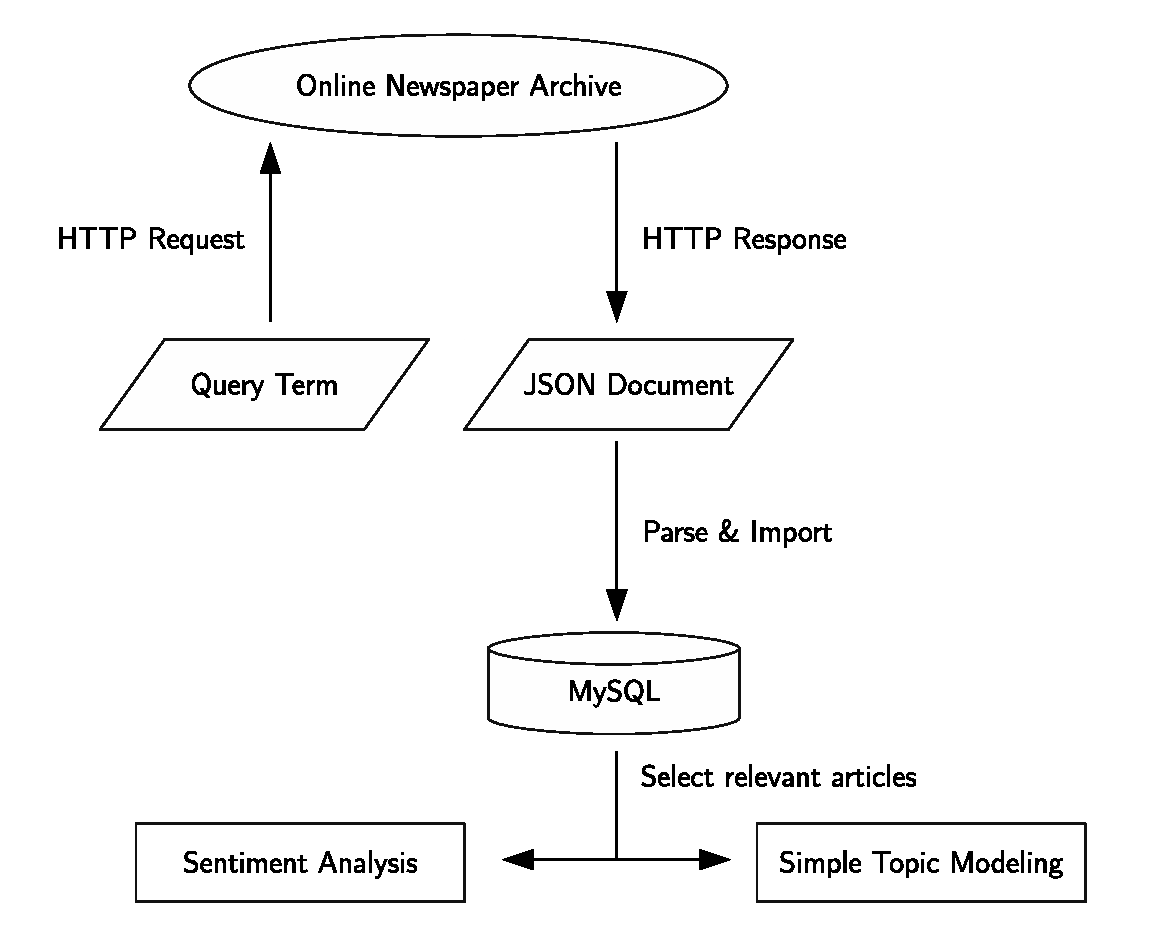
\includegraphics[width=\columnwidth]{figures/workflow_eps}
\caption{Workflow} \label{fig:workflow}
\end{figure}

The analyses are based on two dimensions: query term and time. Thus, the input of the sentiment analysis and our simplified topic modeling approach is a set of paragraphs containing the query term and contained in articles published at a certain time. For instance, such an input can be all paragraphs from the database which contain the word \textit{homosexual} and where published in the 1990s. The sentiment analysis assigned each sentence a vector of sentiment probabilities. We considered five sentiments: \textit{very negative}, \textit{negative}, \textit{neutral}, \textit{positive}, and \textit{very positive}. The vector $\langle 0.2, 0.5, 0.1, 0.1, 0.1\rangle$, for instance, describes the case that a sentence has a probability of $20\%$ for being very negative, $50\%$ for being negative, and $10\%$ for being neutral, positive, and very positive, respectively. For topic modeling, the joint occurrence of a target term together with another word (cooccurrence) is analyzed. Target terms are LGBT-related words, like the query terms. Each cooccurrence is assigned its frequency and whether its occurrence is significant. For instance, the cooccurrence $c_\text{2010s} = \langle \text{bisexual}, \text{rights}, 31, \text{true}\rangle$ means that within the paragraphs from 2010 to 2019, \textit{bisexual} and \textit{rights} occurred 31-times in the same paragraph and that this occurrence is significant. By clustering significant cooccurrences, the topics were manually created in order to yield high-quality topics.

\paragraph*{Implementation} The whole workflow is implemented in Java as a Maven\footnote{\url{https://maven.apache.org/}} project. The project is managed on GitHub.\footnote{https://github.com/macksimiljan/lgbt-news} It consists of one module for collecting and one for analyzing the data. The database is accessed by using the Java Database Connectivity (JDBC) API. The used query terms are \textit{bisexual}, \textit{gay community}, \textit{homosexual}, \textit{lesbian}, \textit{transgender}, and \textit{transsexual}. However, the term \textit{gay} was not considered as a query term because it appeared too often in non-LGBT-related contexts like as a given name or surname. In order to obey the time limit of the NYT API, only one request per second was sent. Almost all requests ($95.4\%$) were successful. They returned a non-empty JSON object which could be inserted into the database. Failures of requests were due to denied accessed to the archive (HTTP 403) or gateway time-outs (HTTP 504). Because such failures were very rare, failed requests were not sent for a second time. All in all, the built corpus consists of $44,485$ articles whereby $93,7\%$ of them contain a non-empty lead paragraph on which the analyses are based.

The database models the mapping of query terms and keywords to articles. Keywords represent interesting additional information to the articles like associated persons, organizations, or geographical information. Approximately, $75\%$ of all articles have at least one keyword. Moreover, an article has a URL which leads to its HTML representation in two-thirds of the cases; otherwise the article is only accessible as a PDF document.\footnote{Older articles are archived as PDF not as HTML.} Further attributes are the publication date, the actual text type (for instance, article, interview, or biography) and headline, abstract, lead paragraph, and snippet. Since the headline is very short, the abstract is missing for $62\%$ of the articles, and the snippet is mostly the same as the lead paragraph, the analysis is based on the lead paragraph.

Essentially, the analysis module of the Maven project comprises the sentiment and the topic model package. They both rely on the sentence extraction task. For a certain search word and a certain publication date, this task selects windows of sentences from the paragraphs in the database. The window size is parameterized, i.e.,  Both of them depend on the natural language processing library Stanford CoreNLP\footnote{\url{http://stanfordnlp.github.io/CoreNLP/}}. This library contains annotators for tokenization, sentence splitting, part-of-speech tagging, and sentiment analysis. 


//TODO: keyword analysis

\section{Underlying Data}
%The data underlying the sentiment and topic analysis are newspaper articles from the New York Times (NYT) and the Guardian. They were accessed by the NYT Article Search API\footnote{LINK} and by XYZ\footnote{LINK}. The returned data were stored in a MySQL database. A relational database allows a quick access of the data along with a powerful query language for data summarization whereas the APIs have limited access and no in-depth and flexible summarization options. The NYT API, for instance, enables requesting only 10 articles per second but not more than $10\cdot 10^3$ per day and per API key. Consequentyl, the articles had to be exported from the newspaper archives before the analysis was executed. Neither the API of the NYT nor of the Guardian returned the fulltext article but both returned an URL to it. \textit{// wollen wir diesen link auch abrufen?} For NYT, this link leads to the actual article in 2/3 of the cases; otherwise the full article was not accessible because, for instance, it had to be bought. Nevertheless in all most all cases, the NYT API response consisted of a snippet and lead paragraph for the particular article. Furhter attributes which are analysed later on are the publication date, the publication type\footnote{Most the publicated texts are articles but there are interviews, biographies, editorials and others. However, all of these texts are called articles in this current thesis when the actual type is irrelevant.}, the number of words within the article as well as keywords like geographical location or subject.
%
%The workflow for requesting and storing the articles has been implemented in Java as a Maven project. Almost all requests ($98.4\%$) were successful. They returned a non-empty JSONObject which was parsed and inserted into the database via JDBC. The requests failed due to HTTP 403 (REASON) or 504 (REASON). All in all, the database contains $00,000$ articles from NYT and $00,0000$ from the Guardian. The number of articles per query term and newspaper is shown in Tab.\ref{tab:noOfArticles}. The last part of this section presents the query terms for the articles. \textit{// gibt es artikel, die mehreren query terms zugeordnet sind?}
%
%\begin{table}
%\centering
%\caption{Article count per newspaper.}
%\label{tab:noOfArticles}
%\begin{tabular}{lcc}
%\toprule
%query term & NYT & Guardian\\
%\midrule
%homosexual & $15,086$ & \\
%\bottomrule
%\end{tabular}
%\end{table}


%\subsection*{Homosexual}
%There are approximately $15 \cdot 10^3$ articles containing the term `homosexual' in the NYT archive. All of them are assigned with a publication date. Although there is at least one article which is published within a decade from 1910 onwards, the term frequently occured in the 1970s for the first time, see Fig.\ref{fig:histo-homosexual-nyt}. In 1940s, the more than 4000 articles containing this term where published. In the next three decades the its frequency has decreased. \textit{// why?} $82.5\%$ of all articles are either of type news, article, or review. Only $5\%$ has a geographical information. 

%\subsection*{Lesbian}
%
%\subsection*{Same-Sex}

\section{Results}

\subsection{Sentiment Analysis}
This is our spectacular sentimental analysis.

\subsection{Simple Topic Modeling}
This is our great topic modeling.

\section{Discussion}
This is our insightful discussion.
\subsection{Implementation Issues}

\subsection{Content Issues}

\subsection{Future Work}

\section{Conclusion}
This is our awesome conclusion.

\end{document}